\documentclass{article}
\usepackage[right=20mm,left=20mm,top=20mm,bottom=15mm]{geometry}
\usepackage[utf8]{inputenc}
\usepackage{babel}
\usepackage{graphicx}
\usepackage{tikz}
\usepackage{booktabs}
\usepackage{listings}
\usepackage{xcolor}
\lstset{
  basicstyle=\ttfamily\small,
  breaklines=true,
  frame=single,
  columns=fullflexible,
  keepspaces=true,
  tabsize=4,
  language=Java,
  keywordstyle=\color{blue}\bfseries,
  commentstyle=\color{gray},
  stringstyle=\color{orange},
}
\usepackage{longtable}
\usepackage{hyperref}
\usepackage{fancyhdr}
\usepackage{float}
\geometry{margin=2.5cm}
\pagestyle{fancy}
\fancyhf{}
\rhead{Proyecto syntx}
\rfoot{\thepage}

\title{Informe de rendimiento y presentación del Motor Léxico \texttt{syntx}}
\author{XXXXXXXX, abril de 2025}
\date{}

\begin{document}

\maketitle

\section*{Resumen}

Este documento presenta un informe detallado sobre el rendimiento y el consumo de memoria del motor léxico \texttt{syntx}, diseñado con un enfoque modular, predictivo y extensible para múltiples lenguajes de programación. Se incluyen comparaciones con herramientas consolidadas como \texttt{javalang}, \texttt{tree-sitter}, \texttt{rustc\_lexer}, entre otras.
Este motor léxico surgió originalmente como una herramienta auxiliar para el sistema de construcción \texttt{jmake}, donde se requería un análisis léxico rápido y seguro para resolver dependencias de forma incremental. Su diseño modular y expresivo motivó su separación como proyecto independiente.
\section*{Demostración de Abstracción sin Coste en Rust}

Una de las propiedades clave del diseño del motor \texttt{syntx} es que permite una integración directa con cualquier conjunto léxico mediante el sistema de tipos de Rust, sin incurrir en sobrecoste de ejecución. A continuación se muestra un ejemplo funcional mínimo:

\begin{verbatim}
use syntx::engine::Lexer;
use syntx::langs::java::JavaTokenSet;

let mut lexer = Lexer::<JavaTokenSet>::from_str(source_code);
lexer.tokenize();
\end{verbatim}
\\
Gracias al sistema de tipos y la tecnología de genéricos de Rust, el motor es \textbf{completamente modular}: el mismo \texttt{Lexer<T>} puede adaptarse a distintos lenguajes sin modificar el motor ni reconfigurar el flujo de ejecución. El usuario puede definir un nuevo lenguaje implementando únicamente 5 o 6 funciones sobre un tipo \texttt{T} que cumpla los traits \texttt{Lexable} y \texttt{Delimeted}, junto con una definición manual de su conjunto de tokens. Esto permite que los tokens sean altamente expresivos, personalizados y ajustados a las necesidades gramaticales del lenguaje objetivo.

\subsection*{Estructura del Lexer}

\begin{verbatim}
#[derive(Debug)]
pub struct Lexer<'a, T: Lexable + Delimeted + Eq + Hash + Clone> {
    pub tokens: Vec<T::Token>,
    pub contents: Peekable<Chars<'a>>,
    pub state: State<T>,
}
\end{verbatim}
\\
El analizador léxico mantiene un buffer de tokens generados (por ahora), una vista previa sobre los caracteres del código fuente, y una estructura de estado interna parametrizada por el tipo del lenguaje (Autómata Finito con conocimiento de coordenadas, niveles de indentación y contexto en tiempo real). No hay necesidad de usar \texttt{Box}, punteros dinámicos ni almacenamiento en heap adicional. Todo el trabajo es resuelto en tiempo de compilación mediante especialización monomórfica.

\section*{Representación de Gramáticas mediante Árboles Ponderados con Reserva de Memoria en Arena}

El motor \texttt{syntx} utiliza una estructura de árbol genérica altamente optimizada, pensada para almacenar reglas sintácticas y caminos de predicción léxica además de un futuro AST. Cada nodo es almacenado en memoria continua usando el allocator \texttt{bumpalo}, lo cual permite una inserción masiva y constante sin realocaciones dinámicas individuales.

\subsection*{Definición de la Estructura en Rust}

\begin{verbatim}
#[derive(Debug)]
pub struct Node<'bump, T>
where
    T: std::hash::Hash + std::cmp::Eq + Clone,
{
    pub leafs: AHashMap<T, &'bump RefCell<Node<'bump, T>>>,
    pub left: Option<&'bump RefCell<Node<'bump, T>>>,
    pub right: Option<&'bump RefCell<Node<'bump, T>>>,
    pub is_ast_node: bool,
    pub weight: usize,
    pub value: Option<T>,
    pub end: bool,
}

#[derive(Debug)]
pub struct Tree<'bump, T>
where
    T: Hash + Eq + Clone,
{
    pub arena: &'bump Bump,
    pub cursor: &'bump RefCell<Node<'bump, T>>,
    pub root: &'bump RefCell<Node<'bump, T>>,
    pub stack: BVec<'bump, &'bump RefCell<Node<'bump, T>>>,
}
\end{verbatim}

\textbf{Resumen técnico:}
\begin{itemize}
    \item Cada nodo (\texttt{Node}) representa un valor gramatical (terminal o no terminal) y apunta a un conjunto de hijos mediante un \texttt{AHashMap}.
    \item Todos los nodos viven en una \texttt{arena} compartida (\texttt{bumpalo::Bump}), lo que minimiza la fragmentación.
    \item El árbol soporta navegación por cursor y backtracking mediante una pila interna.
\end{itemize}

\subsection*{Ventajas del Diseño}

\begin{itemize}
    \item La inserción de nuevas ramas se realiza en tiempo constante, al igual que el desplazamiento transversal y backtracking.
	\item Toda la estructura vive en una sola asignación de memoria, lo cual mejora la localidad de caché, además de solventar problemas de tiempo de vida de la memoria en el \textbf{Heap}, de lo cual se ocupa el \textbf{Borrow Checker} de rust, ya que syntx está pensado desde un punto de vista \textbf{seguro} que no dé lugar a leaks de memoria.
    \item Facilita la serialización, visualización, y exportación de gramáticas formales.
\end{itemize}

\newpage{}
\section*{Evaluación sobre Código Java}

\textbf{Archivo utilizado:} \texttt{DataBaseMetadata.java (NASA JMARS)}

\begin{verbatim}
========== Resultados del Benchmark ==========
Líneas        : 8094  
Tokens        : 35126  
Tiempo        : 0.0048 s  
Memoria       : 1.31 MB  
Líneas/seg    : 1.697.167  
Tokens/seg    : 7.365.293  
\end{verbatim}
\\
\textbf{Observación:} El motor demuestra una velocidad equiparable a analizadores léxicos utilizados en compiladores como \texttt{rustc}, con un uso mínimo de memoria.

\section*{Evaluación sobre Código en C}

\textbf{Archivo utilizado:} \texttt{decode.c (FFmpeg src)}

\begin{verbatim}
========== Resultados del Benchmark ==========
Líneas        : 2223
Tokens        : 11072
Tiempo        : 0.0019 s
Memoria       : 0.38 MB
Líneas/seg    : 1.146.113
Tokens/seg    : 5.708.399
\end{verbatim}
\\
\textbf{Observación:} El lexer mantiene su rendimiento en código C real con alta densidad léxica y estructuras complejas.

\section*{Comparativa de Thoughput entre Lexers}

\begin{table}[H]
\centering
\begin{tabular}{@{}llll@{}}
\toprule
\textbf{Herramienta} & \textbf{Implementación} & \textbf{Tokens/seg} & \textbf{Características principales} \\
\midrule
StreamTokenizer       & Java        & 679.000     & Mínima sensibilidad gramatical \\
javalang              & Python      & 290.000     & Parser completo de Java        \\
pylyzer               & Python      & 200.000     & Sensible a espacios y estructura \\
tree-sitter           & C/Rust      & 1.060.000   & Análisis sintáctico por gramáticas \\
rustc\_lexer           & Rust        & 17.662.500  & Nativo (sin inferencia) \\
TypeScript Lexer      & TypeScript  & 750.000    & Lexer oficial del compilador TypeScript \\
Acorn (JavaScript)    & JavaScript  & 729.000     & Lexer modular basado en AST minimalista \\
\textbf{syntx}        & Rust        & \textbf{7.165.668} & Lexer predictivo y modular \\
\bottomrule
\end{tabular}
\caption{Aproximación de rendimiento en análisis léxico (tokens por segundo)}
\end{table}

\vspace{1em}
\noindent \textbf{Conclusión técnica:}
\begin{itemize}
    \item \texttt{syntx} alcanza un rendimiento comparable a \texttt{rustc\_lexer} con una arquitectura extensible.
    \item Su uso de memoria es inferior al de la mayoría de herramientas de análisis existentes.
    \item El diseño permite su integración en compiladores, analizadores estáticos e IDEs.
\end{itemize}

\section*{Comparativa de Uso de Memoria}

\begin{table}[H]
\centering
\begin{tabular}{llllll}
\toprule
\textbf{Lenguaje} & \textbf{Archivo} & \textbf{Memoria (MB)} & \textbf{Tokens} & \textbf{Tiempo (s)} & \textbf{Tokens/seg} \\
\midrule
Java & DataBaseMetadata.java & 1.31 & 35126 & 0.0048 & 7.365.293 \\
C    & decode.c & 0.38 & 11072 & 0.0019 & 5.708.399 \\
\bottomrule
\end{tabular}
\caption{Comparación del uso de memoria entre lenguajes}
\end{table}

\section*{Consideraciones Técnicas}

\begin{itemize}
    \item Las mediciones fueron realizadas con compilaciones optimizadas mediante \texttt{cargo run --release}.
    \item El uso de memoria fue obtenido desde \texttt{/proc/<pid>/statm} (Linux).
    \item Todas las pruebas incorporaron límites estrictos de tiempo y memoria como validación.
    \item El lexer está diseñado para un comportamiento determinista y eficiente en proyectos de gran escala.
\end{itemize}


\begin{figure}[H]
\centering
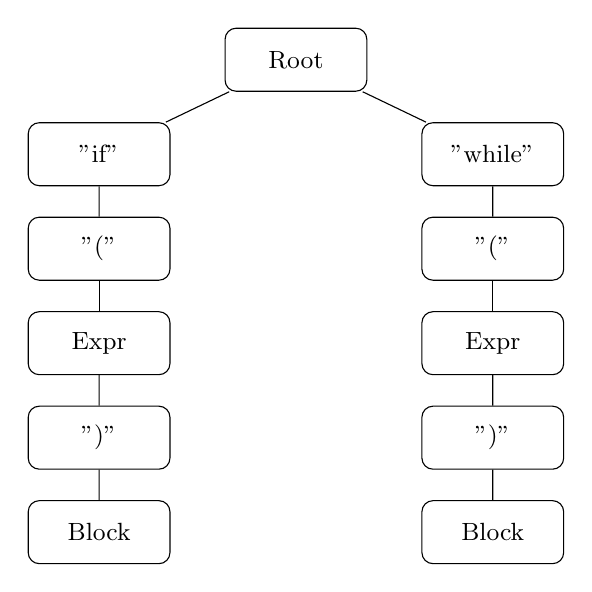
\begin{tikzpicture}[
  level distance=1.2cm,
  every node/.style={draw, rounded corners, minimum width=1.8cm, minimum height=0.8cm, font=\small},
  level 1/.style={sibling distance=5cm},
  level 2/.style={sibling distance=3.2cm},
  level 3/.style={sibling distance=2.4cm},
  level 4/.style={sibling distance=2cm}
]

\node {Root}
  child { node {"if"}
    child { node {"("}
      child { node {Expr}
        child { node {")"}
          child { node {Block} }
        }
      }
    }
  }
  child { node {"while"}
    child { node {"("}
      child { node {Expr}
        child { node {")"}
          child { node {Block} }
        }
      }
    }
  };

\end{tikzpicture}
\caption{Árbol de producción sintáctica almacenado en arena}
\end{figure}

\section*{Planes a futuro}

Se identifican múltiples direcciones de desarrollo posibles para expandir la funcionalidad y robustez del motor léxico y sintáctico \texttt{syntx}:

\begin{itemize}
  \item Propagación de errores de sintaxis antes de llegar a fases avanzadas de creación de ASTs.
  \item Predicciones deterministas guiadas por pesos ajustados dinámicamente durante la interpretación léxica.
  \item Arquitectura multi hilo con buffers de datos compartidos para maximizar el paralelismo en la tokenización.
  \item Implementación de algoritmos \textit{fuzzy} para predicción de errores y tolerancia a errores sintácticos en entradas parciales.
  \item Análisis incrementales mediante uso de hashes funcionales en lugar de sintácticos para evitar trabajo redundante.
  \item Generación de tokens especializada para lenguaje natural, con inferencia de tipos gramaticales y sintácticos orientada a tareas de aprendizaje automático.
  \item Métodos de inserción automática de rutas gramaticales en el árbol mediante reglas inferidas o declarativas.
\end{itemize}

\section*{Ventajas de los Enum Wrappers en Rust}

Una de las características más poderosas del ecosistema de tipos en Rust es la capacidad de modelar estructuras léxicas complejas mediante enumeraciones anidadas y envueltas, también conocidas como \textit{enum wrappers}.
\\
Este patrón permite definir tokens jerárquicos que encapsulan variantes dentro de otras variantes, preservando información semántica sin sacrificar eficiencia ni seguridad en tiempo de compilación.
\\

\textbf{Ejemplo real de Tokenización para Java:}

\begin{verbatim}
pub enum JavaToken {
    Identifier(JavaIdentifier),
    Operator(JavaOperator),
    Delimeter(JavaDelimeters),
}

pub enum JavaIdentifier {
    Keyword(Keyword),
    CharLiteral(String),
    StringLiteral(String),
    Integer(String, JavaBase),
    Unknown(String),
}
\end{verbatim}
\\
Gracias a esto, el lexer puede producir un flujo de tokens altamente expresivo y preciso, manteniendo toda la información relevante para las fases posteriores de análisis. Además, al estar resuelto en tiempo de compilación mediante variantes concretas.
\\
Este enfoque también permite un tipo de coincidencia exhaustiva con \texttt{match} que mejora la legibilidad, mantenibilidad y seguridad del compilador o analizador sintáctico que lo utilice.
\\
Este algoritmo predictivo se implementa sin costo adicional de memoria, ya que el iterador es clonado superficialmente y no se incurre en copia profunda del contenido.

\section*{Demostración de expresividad léxica con enums anidados}

Para ilustrar la riqueza semántica de los tokens generados por el motor, se muestra a continuación un fragmento reducido de código Java junto a su representación tokenizada mediante enums anidados (la identificacion de tipos primitivos en lenguajes altamente tipados está en desarrollo):

\begin{lstlisting}[language=Java, caption=Demo.java - Fragmento simple con riqueza léxica]
public class Demo {
	public static void main(String[] args) {
		int x = 42;
		String msg = "Hola\nMundo";
		if (x >= 10) {
			System.out.println(msg);
		}
	}
}
\end{lstlisting}
\newpage{}
\noindent \textbf{Tokens generados:} \hfill (Identificadores como Strings para claridad, normalmente normalizados)

\begin{verbatim}
Identifier(Keyword(Public))
Identifier(Keyword(Class))
Identifier(Unknown("Demo"))
Delimeter(LBrace)
Identifier(Keyword(Public))
Identifier(Keyword(Static))
Identifier(Keyword(Void))
Identifier(Unknown("main"))
Delimeter(LParen)
Identifier(Unknown("String"))
Delimeter(LBracket)
Delimeter(RBracket)
Identifier(Unknown("args"))
Delimeter(Rparen)
Delimeter(LBrace)
Identifier(Keyword(Int))
Identifier(Unknown("x"))
Operator(Assign)
Identifier(Integer("42", Decimal))
Delimeter(Semicolon)
Identifier(Unknown("String"))
Identifier(Unknown("msg"))
Operator(Assign)
Identifier(StringLiteral("Hola\nMundo"))
Delimeter(Semicolon)
Identifier(Keyword(If))
Delimeter(LParen)
Identifier(Unknown("x"))
Operator(Geq)
Identifier(Integer("10", Decimal))
Delimeter(Rparen)
Delimeter(LBrace)
Identifier(Unknown("System"))
Operator(Dot)
Identifier(Unknown("out"))
Operator(Dot)
Identifier(Unknown("println"))
Delimeter(LParen)
Identifier(Unknown("msg"))
Delimeter(Rparen)
Delimeter(Semicolon)
Delimeter(RBrace)
Delimeter(RBrace)
Delimeter(RBrace)
\end{verbatim}
\\
Este ejemplo demuestra cómo una única pasada del lexer puede clasificar y jerarquizar información léxica compleja mediante enums anidados, permitiendo estructuras de análisis posteriores sin ambigüedad ni pérdida de contexto.

\newpage{}
\section*{Ejemplo de tokenización: caso sintáctico complejo}

\section*{Prueba de esfuerzo: validación del lexer}

Con el objetivo de evaluar la robustez del analizador léxico, usaremos el siguente programa, sintácticamente válido pero deliberadamente complejo, diseñado para maximizar el uso de casos límite: literales binarios y hexadecimales, expresiones ternarias encadenadas, estructuras anidadas en profundidad y combinaciones lógicas de operadores. Este fichero simula un caso límite manteniéndose conforme a la gramática del lenguaje Java.

\begin{lstlisting}[language=Java, caption=Torture.java - Diseñado para poner a prueba el lexer]
public class Torture {
    public static void main(String[] args) {
        int x = 0x1F + 42, y = 0b1010, z = (x << 2) & ~(y | 0xFF);
        String s = "Prepárate: {\n\t¡Lógica intensa!\\\"";
        if (x > y && ((z != 0) ? true : false ? true : false)) {
            System.out.println("¿Por qué harías esto?");
        } else if (x == (y = z = x >>> 1)) {
            s += "Java >>> cordura";
        }
        for (int i = 0, j = 0; i < 10 && j++ < 5; i++) {
            System.out.print((i & j) == 1 ? "*" : ".");
        }
        final int result = x + y + z + (int)(Math.pow(2.5e2f, 1));
        System.out.println("Ω = " + c + " | Resultado = " + result);
    }
}
\end{lstlisting}

\vspace{0.5em}
\noindent
Esta prueba incluye:
\begin{itemize}
    \item Operadores bit a bit: \texttt{\&, |, \textasciitilde, <<, >>>}
    \item Literales hexadecimales y binarios: \texttt{0x1F}, \texttt{0b1010}
    \item Literal en coma flotante con notación científica: \texttt{2.5e2f}
    \item Lógica ternaria profundamente anidada
    \item Secuencias de escape en cadenas de texto: \texttt{\\n, \\t, \\\textbackslash}
    \item Asignaciones encadenadas y bucles \texttt{for} con múltiples variables
\end{itemize}

\subsection*{Resumen del análisis léxico}
\begin{itemize}
    \item Tokens generados: \textbf{185}
    \item Categorías léxicas: \texttt{Keyword}, \texttt{Identifier}, \texttt{Operator}, \texttt{Delimeter}, \texttt{Literal}
    \item Cadenas escapadas y sufijos numéricos identificados correctamente
\end{itemize}

\subsection*{Métricas de rendimiento}
\begin{itemize}
    \item Tiempo de ejecución: \textbf{0.0000 s} \hfill (\texttt{time target/release/syntx})
    \item Memoria: \textbf{0.12 MB}
    \item Líneas por segundo: \textbf{490.990}
    \item Tokens por segundo: \textbf{4.541.660}
\end{itemize}

\appendix
\section*{Anexo: Especificaciones técnicas del motor "under the hood"}
El motor \texttt{syntx} implementa un conjunto de estrategias específicas para lograr un equilibrio entre rendimiento, expresividad y seguridad en tiempo de compilación. A continuación se detallan algunas de las decisiones clave en su arquitectura interna:

\subsection*{Reconocimiento de secuencias de comentarios mediante lectura predictiva}

El reconocimiento de secuencias compuestas de comentarios se realiza siguiendo una estrategia \textit{greedy} basada en el principio de \textit{maximal munch}. El lexer clona superficialmente el iterador de entrada y lee la mayor secuencia posible de caracteres que coincida con una secuencia válida, deteniéndose en el primer fallo. Esta técnica permite distinguir correctamente entre símbolos como \texttt{//}, \texttt{/**}, \texttt{/*} y \texttt{///!}, sin necesidad de lookahead explícito ni retroceso.

\subsection*{Gestión de memoria sin heap tradicional}

No se utilizan asignaciones dinámicas convencionales como \texttt{Box} o \texttt{Rc}. En su lugar, toda la memoria dinámica requerida por las estructuras de árbol es gestionada mediante el allocator \texttt{bumpalo}, garantizando inserciones constantes, sin fragmentación, y con un modelo de propiedad sencillo de verificar por el compilador.

\subsection*{Separación de responsabilidades}

La lógica léxica (tokenización) y la lógica gramatical (predicción estructural) están desacopladas. El lexer opera únicamente sobre la entrada y genera un flujo de tokens, mientras que el árbol de predicción gestiona rutas válidas sin intervenir en la lectura de caracteres. Esto permite probar y extender ambos subsistemas por separado.

\subsection*{Sin introspección de tipos en tiempo de ejecución}

Toda la estructura de tipos es conocida y validada en tiempo de compilación, permitiendo optimizaciones agresivas por parte del compilador y evitando ramas condicionales innecesarias para lenguajes fuertemente tipados.

\subsection*{Lectura inmutable del input}

El lexer nunca copia ni muta el código fuente. Trabaja sobre un iterador de caracteres por referencia, lo cual minimiza el uso de memoria y garantiza acceso seguro sin duplicaciones. Esto permite tokenizar archivos de gran tamaño con un perfil de memoria mínimo.

\subsection*{Reducción de ruido en el flujo de tokens}

El lexer almacena únicamente los tokens léxicamente relevantes. No conserva espacios, tabulaciones ni otros caracteres triviales para lenguajes en los que tales elementos no afectan la interpretación semántica. Esta decisión permite reducir el uso de memoria, disminuir el tiempo de inserción de tokens, y evitar análisis adicionales innecesarios.
\\
En este sentido, el comportamiento del lexer es analógico al de un filtro de paso bajo: elimina el “ruido” superficial del código fuente y transmite únicamente la señal estructural que alimenta al árbol gramatical y a las etapas posteriores de análisis.
\vfill
\begin{center}
\small Abril de 2025 - Proyecto \texttt{syntx}, motor léxico, modular y predictivo de alto rendimiento - XXXXXXXX@XXXXXX
\end{center}

\end{document}
